\documentclass[a4paper,conference]{IEEEtran}

\usepackage{amsmath}
\usepackage{graphicx}

\begin{document}

\title{Genetic Painting}
\author{\IEEEauthorblockN{Liangwang Ruan}
  \IEEEauthorblockA{Peking University\\
  Email: ruanliangwang@pku.edu.cn\\
  Student ID: 2101111577}}
\maketitle

\begin{abstract}
  The abstract goes here.
\end{abstract}
\section{Introduction}
Generative art refers to art that in whole or in part has been created with the use of an autonomous system, has been widely studied over the past decades. A specific branch of generative art uses computer algorithms to show(most visually) regularity of mathematical patterns and show variability from pseudo-random numbers, it's known as algorithmic art. A typical example of algorithmic art is fractal art as shown in Fig. \ref{fig:fracal}.

\begin{figure}[htp]
  \centering
  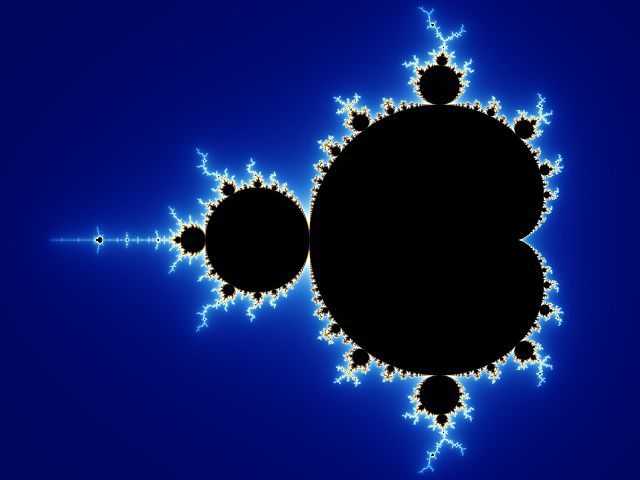
\includegraphics[width=.8\columnwidth]{imgs/mandelbrot_set.jpg}
  \caption{Mandelbrot Set \copyright From Wikipedia}
  \label{fig:fracal}
\end{figure}

Intelligent optmization algorithms are espeically designed to deal with NP-hard, non-convex, non-smooth optmization problems, the complexity of the problems and the bionics nature of intelligent 

\section{Related Work}

\subsection{Genetic Algorithm}

\subsection{Procedure Painting}

\section{Algorithm}


\end{document}